\documentclass{article}
\usepackage{graphicx}
\usepackage{booktabs}
\usepackage{tabularx}

\title{Development Plan\\\progname}

\author{\authname}

\date{}

%% Comments
\usepackage{color}
\newif\ifcomments\commentstrue %displays comments
%\newif\ifcomments\commentsfalse %so that comments do not display
\ifcomments
\newcommand{\authornote}[3]{\textcolor{#1}{[#3 ---#2]}}
\newcommand{\todo}[1]{\textcolor{red}{[TODO: #1]}}
\else
\newcommand{\authornote}[3]{}
\newcommand{\todo}[1]{}
\fi
\newcommand{\wss}[1]{\authornote{blue}{SS}{#1}} 
\newcommand{\plt}[1]{\authornote{magenta}{TPLT}{#1}} %For explanation of the template
\newcommand{\an}[1]{\authornote{cyan}{Author}{#1}}
%% Common Parts
\newcommand{\progname}{4TB6 - Mechatronics Capstone} % PUT YOUR PROGRAM NAME HERE
\newcommand{\authname}{Team \#5, Locked \& Loaded
\\ Abi Nevo, nevoa
\\ Elsa Bassi, bassie
\\ Steffi Ralph, ralphs1
\\ Abdul Iqbal, iqbala18
\\ Stephen De Jong, dejons1
\\ Anthony Shenouda, shenoa2} % AUTHOR NAMES                  

\usepackage{hyperref}
    \hypersetup{colorlinks=true, linkcolor=blue, citecolor=blue, filecolor=blue,
                urlcolor=blue, unicode=false}
    \urlstyle{same}


\begin{document}
\maketitle
\begin{figure}[h!]
  \centering
  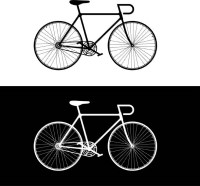
\includegraphics[width=0.4\linewidth]{../BikeLogo.jpg}
\end{figure}

\begin{table}[hp]
\caption{Revision History} \label{TblRevisionHistory}
\begin{tabularx}{\textwidth}{llX}
\toprule
\textbf{Date} & \textbf{Developer(s)} & \textbf{Change}\\
\midrule
Sept 25 & Abi & Drafted Team Meeting, Communication Plan, \& Team Member Roles\\
Sept 26 & Elsa & Drafted Workflow Process\\
Sept 26 & Stephen & Drafted Intro, Demo Plan, \& Scheduling\\
Nov 10 & Steffi & Updated Development Plan, \& Technology\\
\bottomrule

\end{tabularx}
\end{table}

\newpage



\section{Introduction}

The Smart Lock will be the first model of smart bike locks produced by Locked \& Loaded. The lock will be mounted to your favourite bike with many features that can be controlled from a smart phone. Additionally other outputs may be monitored such as the lock state, battery level and position.

\section{Team Meeting Plan}

Our team will have a meeting weekly on Mondays at 10:30 AM in Thode library.  Should we decide on Monday that we need another meeting that week, we will have a meeting on Thursdays at 2:30 PM, also in Thode.  If more meeting time is still necessary, our group will arrange for a meeting on Friday or over the weekend.

Meetings with our supervisor, Dr. Sirouspour, will occur biweekly (once every two weeks) on Wednesdays from 11 AM to 12 PM virtually via Teams.

An agenda will be created and committed to our Git repo prior to meetings.  This responsibility will be assigned to a different team member each week, on a rotation, however, all team members may suggest agenda topics.  The agenda will include suggested meeting topics, who will present/lead each topic, and an estimated time of discussion. Meeting minutes will also be recorded in the same document as the agenda, by the same team member, and be uploaded to our Git repo after the meeting.  This team member will also be responsible for chairing the meeting. 

\section{Team Communication Plan}

Our primary form of fast, short communication will be through our text group chat. We will use Github to post issues and host documentation for deliverables.  In addition to Github, we will also use Trello for project management and task tracking (Kanban).  Lastly, we will use Teams to host virtual meetings.

\section{Team Member Roles}

\begin{table}[h]
\caption{Team Member Roles} \label{TblTeamMemberRoles}
\begin{tabularx}{\textwidth}{llX}
\toprule
\textbf{Role} & \textbf{Primary Lead} & \textbf{Support}\\
\midrule
Embedded Systems Design & Elsa & Abi\\
Documentation/Latex/"Faux Marker"/Git & Steffi & Elsa\\
Lock Frame Design (CAD) & Stephen & Steffi\\
Software (App Development) & Anthony & Abdul\\
Software (Wireless Communication) & Abi & Anthony\\
Lock Mechanism Design (CAD) & Abdul & Stephen\\
\bottomrule
\end{tabularx}
\end{table}

Each member has been designated as a lead for the various features/topics of our project, however, each member should have some knowledge of every aspect.  Team members should be prepared to be flexible and give support to whichever aspect/feature has current need. 

\section{Workflow Plan}

\subsection{Code Development}

Team members are expected to use the team repository on Github for code development. The master branch will be used as the current working copy of the code. To develop code, they will fork the main branches to create sub-branches that can then be merged back to the main branch according to the rules outlined below. 

\subsection{Rules for Merging}

Merging will take place under the following branch protection rules: 

\begin{enumerate}

\item The main branch can only be merged into and not committed to directly. 
\item Merging pull requests is disallowed when tests fail. 
\item Pull requests are required before merging such that one other group member must approve the code. 
\item Status checks and actions must pass before merging. 
\item Branches must be up to date before merging to reduce merge conflicts. 

\end{enumerate} 

\subsection{Commits}

Commits should take place as often as possible, preferably for every 50 lines of code. Commit messages must be specific, concise and descriptive. 

\subsection{Workflow Process}

Our workflow process will be as follows.

\begin{enumerate}
\item Create a detailed and structured plan for the software development. 
\item Pull any new changes from the master branch. 
\item Create a new branch to develop on. 
\item Implement any independent modules. 
\item Perform unit testing on the independent modules. 
\item Push the changes made to the new branch.  
\item Implement any dependent modules .
\item Perform unit testing on the dependent modules.  
\item Merge all changes to the main branch after a pull request is approved by another group member.  
\end{enumerate}

\subsection{Issue Tracking}

Github Issues will be used to track bugs and for accountability purposes. An issue will be created when a developer is unsure about their path forward or if a bug is detected in the code. Issues will be assigned to specific team members explicitly. When an issue is detected and the team member is not able to resolve it themselves, the team lead for that issue will review and advise. Issues can also be raised if a team member foresees a conflict or problem with merging as well as for general tasks. 
\bigskip
They will be categorized according to the following labels.

\begin{itemize}

\item Bug: Code that is not working properly.
\item Documentation: Improvements or additions to documentation.
\item Help Wanted: Extra attention is needed.
\item Wontfix: This will not be worked on.
\item CAD: A task related to CAD in this location.
\item Wireless Communications: A task related to wireless communications (i.e., Bluetooth, GPS) in this location.
\item App: A task related to an application in this location.
\item Embedded Systems Design: A task related to a microcontroller in this location.
\item Stretch Goal: A task related to a stretch goal in this location. 
\item Template: A task related to a template.
\end{itemize}

\subsection{Milestones}

Milestones will be created for each deliverable to keep team members accountable. They will be added continuously as necessary. 

\section{Proof of Concept Demonstration Plan}

Our project requires a large amount of research and development; therefore we must be able to prove that our concept ideas will function as desired and our goals are accomplishable.  We will prove our concept with a demonstration in November.  For our proof-of-concept demo we will produce a prototype of our locking mechanism as well as a crude model of the circuitry that will be required to unlock our mechanism with technology.  We will demonstrate that we are able to complete our objectives with the technologies that exist and that we can understand, and that our physical design will be able to function as desired.  Our demo will be a primary prototype/model and not a final refined version.  

The largest risk we foresee in our project development is our lack of knowledge in wireless communications. In order to complete our project, we first must understand which technologies exactly we must use and implement, then learn how to use those technologies, and finally implement these technologies specifically for our project.  This will have to be a steep learning curve, and we must manage our time effectively in order to complete our project on time. 

Our demo will need to include parts to demonstrate each goal for our product, that with some refinement and revisions will be able to fulfill each requirement of our product. In of our demo, we will need to show the software, hardware and mechanical functionality of our product with models and prototypes.  We will show our code/software through a basic UI that can be utilized on both iOS and Android devices.  To demonstrate our hardware, we will show our selected component and prove that we can accomplish wireless communication as this is a primary requirement for our product to function.  Additionally, we will create a sample circuit which shows the basic functionality of our product and helps to calculate the power requirement that will be necessary.  Finally, to prove that the mechanical design will be functional we will demonstrate the locking mechanism by creating a CAD drawing and prototype it by 3D-printing.  While this is not the only physical component of our product it will be the most technical, therefore, achieving this milestone is a great proof that we will be able to prototype our whole product.  We will also need to test that all the components and devices will be able to communicate and work as an ensemble.  Therefore, the demonstration will touch on how each component will work together to function using the required inputs and giving the desired outputs.


%Our project requires a large amount of research and development, therefore we must be able to prove that our concept ideas will function as desired and our goals are accomplishable. We will prove our concept with a demonstration in November. For our proof-of-concept demo we will need to produce a prototype or model of our system which shows that we will be able to do what we need to do with the technologies that exist, and that our physical design will be able to function as desired. Our demo should be a crude system and not a final refined version.  

%The largest risk we foresee in our project development is our lack of knowledge in wireless communications. In order to complete our project, we first must understand which technologies exactly we must use and implement, then learn how to use those technologies, and finally implement these technologies specifically for our project. This will have to be a steep learning curve, and we must manage our time effectively in order to complete our project on time. 

%Our demo will need to include parts to demonstrate each goal for our product and that with some refinement and revisions we will be able to fulfill each requirement. For implementation of our demo, we will need to show the software, hardware and mechanical functionality of our product with models and prototypes. We will show our code/software through a set of test cases or utilizing a model. For our hardware we will need to demonstrate that the components will be able to complete our tasks, using a sample circuit to prove the technology works. Finally, for the mechanical design as well as packaging of our product we will need to simulate design using CAD software and prototype using 3d-printing, laser cutting, or manual construction. We will also need to test that all the components and devices will be able to communicate and work as an ensemble. Therefore, we will demonstrate that the system is able to function using the required inputs and giving the desired outputs.

\section{Technology}

The mobile application will be developed in the Visual Studio Environment using the Flutter framework in order to allow for cross-platform development.  Within Flutter, the development language used will be Dart and a DartLint will be used to maintain the code throughout the evolution of the code.  Finally, for the mobile application development/testing XCode will be used to emulate iOS devices and Android Studio will be used to emulate Android devices. 

%The mobile application will be developed using XCode Ver.14.0 IDE, utilizing the Swift programming language for iOS Development. A limitation of this platform is that it only allows for iOS development. The Flutter IDE could be used as an extension as it allows for cross-platform development but requires additional research to be used effectively. For linting, we will be using SwiftLint as it is commonly used in the industry for iOS development utilizing XCode. 

The wireless connection between the mobile application and the lock will be accomplished using the Arduino – Nano 33 BLE, via Bluetooth connection.  The coding will be completed in an Arduino IDE using C/C++ languages.

For simple prototyping and early models, the team will 3D print components as it is cheaper and the team as extensive knowledge with the software. Once the model begins to be finalized, parts will be laser cut for higher quality testing. During the prototyping and testing phases, the team will also run FEA analysis to on solid works for free and vigorous testing. The model will also be test in a controlled wet environment for waterproof/weather resistant testing. Multiple sensors, small electric motors, and batteries will also be tested during this phase. Other miscellaneous parts and tooling will be completed in the Hatch Centre as team members have access to the tools and resources there. The team has decided to complete all documentation using Latex and will have them posted on the team Git.

\section{Coding Standard}

The coding style will follow camel case for local variables (lowercaseFirstUpperSecond). Global variables however will follow the same style, but the first word will start with an uppercase letter. Constants and macros will be in full capitals. The code will be modular with functions not being longer than 20 lines of code. Each function will be responsible to complete a single task to enhancing testing and reliability. The functions will also be well commented above the respective function declaration. Also, functions will start with an action verb to describe exactly what the purpose of that function is. For linting, DartLint will be used for enforcing Dart style and conventions.

\section{Project Scheduling}

Our project, work, deliverables, deadlines, and dates will be managed and scheduled accordingly so that our team will be able to complete all tasks and requirement before their due dates. Our team will have weekly meetings in which we will discuss the upcoming dates and deadlines and our goals and strategies to manage them. To manage all our work, we will use various softwares including GitHub milestones and Trello project management. We will post our required tasks and subprojects that need to be completed into GitHub milestones. The GitHub milestones will be associated with a person, a required date of completion, and a set priority. Using this we will be able to see all open issues for our project and be able to easily delegate them to get our work done. 

	Our major milestones are outlined from the course deliverable schedule, with the Proof of Concept Demo, Revision 0 Demo, Final Demo, \& Final Documentation being the major milestones. 

	When a larger issue arises, or we are going to tackle a larger problem we will need to be able to split these issues into smaller more manageable ones. To decompose these large tasks, we will modularise our code/functions, utilize small commits, and be intentional with our creation of subbranches. Braking things up in terms of the skills, technologies, and knowledge required to complete each task. We will all need/be able to work on each issue so it is important to decide who will do what for our team. Each member does have different skills and interests which means tasks will be split in terms of people’s preferences. When tasks can not be split easily, they can be assigned by team lead. Time will need to be managed by all team members knowing that everyone has a lot of other requirements and priorities.

\end{document}
